\chapter{Introduction}
The ability to communicate with the user in a natural language is a major driving
force in development of natural language processing algorithms. One of the basic
tasks in a NLP pipeline is parsing by which we can describe sentence structure.
There exist two basic parsing techniques: constituency and dependency parsing.
With constituency parser we break the sentence into phrases, which can be further
broken into smaller sub-phrases. Example of such parsing is shown in figure
\ref{fig:constituency_tree}.

\begin{figure}[!htbp]
  \centering
  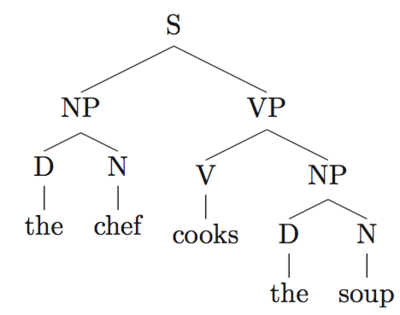
\includegraphics[width=0.4\linewidth]{img/examples/dep/constituent.png}
  \caption{A sample constituency parse tree\todotext{ściągnięte z internetu, przegenerować wektorowo}} 
  \label{fig:constituency_tree}
\end{figure}

In dependency parsing each word (called \emph{dependent})
is connected via labelled arc to another word of the sentence (called \emph{head})
or to the special \emph{ROOT} vertex, forming a directed tree.
Example of such parsing is depicted on figure~\ref{fig:dependency_tree}.

\begin{figure}[!htbp]
  \centering
  \resizebox{0.8\textwidth}{!}{
    \import{img/examples/dep/}{dep.pdf_tex}
  }
  \caption{A sample dependency parse tree} 
  \label{fig:dependency_tree}
\end{figure}

\section{Dependency parsing}

A major advantage of dependency parsers over constituency ones are their
independence from the word ordering. It is important in morphologically rich
languages like Polish or Czech where the ordering is very flexible, and thus
related words can be far apart from each other.
Additionally the head-dependent relationship is a good approximation to semantic
relationship between words~\cite{covington_fundamental_2001} which is important
for tasks like question answering or information extraction.

The labels of head-dependent arcs tells us about grammatical function that
dependent word have in respect to the head. In table~\ref{tab:label_samples}
we show some of the most popular labels for the English language.

\begin{table}[!htbp]
    \centering
    \begin{tabular}{c | c | c}
        Label & Description & Example \\ \hline\hline
        CASE & Case marking & \textit{From} Friday 's Daily \textbf{Star} \\
        NSUBJ & Nominal subject & \textit{Musharraf} \textbf{calls} the bluff \\
        NMOD & Nominal modifier & India \textbf{defensive} over Sri \textit{Lanka} \\
        DET & Determiner & That he missed \textit{a} \textbf{physical} ? \\
        DOBJ & Direct object & Did you \textbf{know} \textit{that} ? \\
        ADVMOD & Adverbial modifier & \textit{So} Bush \textbf{stopped} flying . \\
        AMOD & Adjectival modifier & Six weeks of \textit{basic} \textbf{training} . \\
        COMPOUND & Compound & Bush 's \textit{National} \textbf{Guard} years
    \end{tabular}
    \caption{Most popular labels from English treebank. Dependents are \textit{italic},
    while heads are \textbf{bold}}
    \label{tab:label_samples}
\end{table}

\subsubsection{Projectivity}
We can distinguish two types of dependency trees: projective and nonprojective.
We say that head-dependent arc is projective is there exists a path from head
to every word between head and dependent in the sentence. A dependency tree is
projective if all its arcs are projective.
Intuitively we can say that nonprojective trees are trees that cannot be drawn
without crossing the edges (see figure~\ref{fig:dependency_nonproj}).
Although English dataset has less than 5\% of nonprojective sentences other
languages can have significant amount - like Czech (12\%) or Ancient Greek (63\%)~\cite{straka_parsing_2015}.
It is important to acknowledge this fact because some of the presented parsing
methods can only produce projective trees.

\begin{figure}[!htbp]
  \centering
  \resizebox{1.0\textwidth}{!}{
    \import{img/examples/dep/}{nonproj.pdf_tex}
  }
  \caption{A sample nonprojective dependency parse tree. The on $\rightarrow$ hearing arc is
    nonprojective and thus the whole tree becomes nonprojective.}
  \label{fig:dependency_nonproj}
\end{figure}

\subsection{Parsing algorithms}
In the following section we will present two basic approaches to dependency parsing.
Although they differ in complexity and output flexibility, both of them depend
on supervised machine learning techniques.

\subsubsection{Transition based}
\todotext{Tu będzie łatwiej czytać od "końca"}
In transition based parsing we find a transition sequence from an initial configuration
to a terminal one. A configuration $c$ is a triple $(s, b, A)$ containing stack $s$,
buffer $b$ and set of dependency arcs $A$. For given sentence $w_1, \cdots w_n$
the corresponding initial configuration would be $(\text{[ROOT]}, [w_1, \cdots w_n], \emptyset)$.
The terminal configuration is $(\text{ROOT}, [], A)$ in which $A$ is resulting parse tree.
There are three possible transitions:
\begin{itemize}
    \item {\ttfamily LEFTARC(l)} - Pop from the stack elements $s_1$ and $s_2$,
        add arc $s_1 \rightarrow s_2$ with label $l$ to the set $A$ and push $s_1$ back
        to the stack
    \item {\ttfamily RIGHTARC(l)} - Pop from the stack elements $s_1$ and $s_2$,
        add arc $s_2 \rightarrow s_1$ with label $l$ to the set $A$ and push $s_2$ back
        to the stack
    \item {\ttfamily SHIFT} - Move first element from the buffer to the stack
\end{itemize}
An example of parsing sequence is shown in table~\ref{tab:transition_parse}.
\begin{table}[!htbp]
    \centering
{\footnotesize
    \begin{tabular}{l | l | l | l}
        Stack & Buffer & Transition & New arcs \\ \hline
        $[$ROOT$]$ & $[$He has good control$]$ & {\ttfamily SHIFT} & - \\
        $[$ROOT He$]$ & $[$has good control$]$ & {\ttfamily SHIFT} & - \\
        $[$ROOT He has$]$ & $[$good control$]$ & {\ttfamily LEFTARC(nsubj)} & nsubj(has,He) \\
        $[$ROOT has$]$ & $[$good control$]$ & {\ttfamily SHIFT} & - \\
        $[$ROOT has good$]$ & $[$control$]$ & {\ttfamily SHIFT} & - \\
        $[$ROOT has good control$]$ & $[$$]$ & {\ttfamily LEFTARC(amod)} & amod(control, good) \\
        $[$ROOT has control$]$ & $[$$]$ & {\ttfamily RIGHTARC(dobj)} & dobj(has, control) \\
        $[$ROOT has$]$ & $[$$]$ & {\ttfamily RIGHTARC(root)} & root(ROOT, has) \\
        $[$ROOT$]$ & $[$$]$ & - & - \\
    \end{tabular}
}
    \caption{Transitions needed to parse sentence "He has good control"}
    \label{tab:transition_parse}
\end{table}

Because every word of the sentence has be shifted to the stack exactly once
and {\ttfamily ARC} operations reduce stack size by one we will have exactly
$2n$ transitions from initial to terminal configuration, so the time complexity of this
algorithm is $O(n)$ where $n$ is number of words in a sentence.
Using this algorithm we can represent any projective tree 
\cite{nivre_algorithms_2008} (nonprojectives cannot be represented).

The decision which transition to use between consecutive configurations is
obtained through machine learning techniques. This can vary from simple
linear SVM~\cite{nivre_maltparser:_2005} to neural networks~\cite{chen_fast_2014,
andor_globally_2016}.

\subsubsection{Graph based}
Alternative approach is to use graph-based algorithms. The idea is that we define
a space of candidate arcs, find a model that scores each arc and then use some parsing
algorithm to find a final dependency tree with the highest score.

The candidate space and scoring depends on the used learning model.
There exists many parsing algorithms, but one of the most popular is
Chu-Liu-Edmonds \cite{edmonds_optimim_1966}.
The Chu-Liu-Edmonds algorithm, given a directed graph produces minimum spanning
arborescence (minimum spanning tree for directed graph) - it allows us to produce
any parse tree (including nonprojective). The idea is that each vertex chooses 
an incoming edge of minimum weight. If this graph does not contain any cycle then
we are done, else we break the cycle in place that would give us the best result.

Formally the algorithm takes a directed graph $G = (V,E)$, root node $r \in V$,
and weight function $w(e), e \in E$. The algorithm is listed as Algorithm \ref{lst:cle}. 
The standard algorithm has $O(EV)$ running time, but there exist faster implementation
by \cite{gabow_efficient_1986} with $O(E + V\log V)$ running time.

\begin{algorithm}[!htbp]
    \KwData{Directed graph $G$, root node $r$, weight function $w$}
    \KwResult{Spanning arborescence of minimum weight rooted at $r$}
    \Funct{edmonds($G=(V,E)$, $r$, $w$)}{
        Remove any edge from $G$ whose destination is $r$ \;
        For each $v \in V - \{r\}$ find incoming edge of minimum weight, denote it as $\pi(v)$ \;
        Denote new set of edges as $P = {(\pi(v), v) | v \in V - \{r\})}$ \;
        \eIf{$P$ does not contain a cycle}{
            \Return $P$
        }{
            Choose any cycle from $P$ and denote it as $C=(C_v,C_e)$ \;
            Define a new directed graph $G'=(V',E')$, and weighting function $w'$, where $V' = V - C_v + {v_c}$ \;
            Define $E'$ and $w'$ as follows:
            \For{$(u,v) \in E$} {
                \uIf{$u \not\in C_e, v \in C_e$}{
                    $E' = E' + (u, v_c), w'(u, v_c) = w(u,v) - w(\pi(v), v)$
                }
                \uElseIf{$u \in C_e, v \not\in C_e$}{
                    $E' = E' + (v_c, v), w'(v_c, v) = w(u,v)$
                }
                \ElseIf{$u \not\int C_e, V \not\in C_e$}{
                    $E' = E' + (u, v), w'(u,v) = w(u,v)$
                }
                For each new edge remember its origin \;
            }
            Denote $A' = \text{edmonts}(G', r, w')$ \;
            Let $(u, v_c)$ be (unique) incoming edge to $v_c$ in $A'$ \;
            Let $(u,v) \in E (v \in C)$ be a corresponding edge from $G$ \;
            Remove edge $(\pi(v), v)$ from $C$ (breaking the cycle) \;
            Each remaining edge in $C$ together with edges from $E$ that are also present
            in $A'$ forms a minimum spanning arborescence. \;
        }
    }
 \caption{Chu-Liu-Edmonds Algorithm}
 \label{lst:cle}
\end{algorithm}

\subsection{Evaluation of parsing algorithms}
Having predicted dependency tree for a particular sentence we have to be able
to compare it with the gold-standard parse.
There are two main evaluation metrics:
\begin{itemize}
    \item \textbf{Unlabelled Attachment Score} (UAS), is a percentage of words
        with correct predicted head
    \item \textbf{Labelled Attachment Score} (LAS), is a percentage of words
        with correct predicted head \textbf{and} correct predicted label
\end{itemize}
In the experimental section we will show both scores, whenever available.

\subsection{Universal Dependencies}
Up till recently most development of dependency parsers was done in single language
setting, where we have different parser for every language we want to use, each
using language-specific morphosyntactical features. The Universal Dependencies
project \cite{nivre_universal_2015} aims to provide a cross-linguistically consistent
treebank annotation. It is based on previous work on universal Stanford
Dependencies~\cite{marneffe_generating_2006},
Google universal pos tags~\cite{petrov_universal_2011}
and the Interset interlingua~\cite{zeman_reusable_2008}.
The UD project unifies part of speech tags and dependency relations labels
for 30+ languages under common CONNL-U format.
The main advantage is that we can use the same parsing system for every language
(data has consistent format) additionally because the morphosyntactical data has
common format we can try to combine data coming from different languages (see
section~\ref{sec:neural_multilingual}).

\section{Neural Networks}
A neural network is a mathematical model loosely based on how brain works.
%A typical, simple model consists of few layers, each containing many neurons.
%Each neuron has incoming connections from previous layer and outgoing to the
%next layer. Each neuron computes weighted sum of its input ......
The models proven to be very flexible and obtained state of the art results in
many tasks like machine translation~\cite{bahdanau_neural_2014},
caption generation~\cite{xu_show_2015} or image recognition~\cite{szegedy_goglenet_2014}
A neural network is defined by its topology,
activation functions and parameters. The first two are chosen by the author,
while the parameters are obtained by learning procedure.

The topology of the network is telling us how the layers of neurons are connected
to each other. Each layer have a number of neurons which have some incoming
indices $i$, associated activation function $\phi$ and some parameters $w$.
The neuron combines the incoming signals, usually by taking weighted average
and then applying the activation function: $ \phi ( \sum_{k=0}^{|i|} w_ki_k ) $.
This value is then feeded to the connected neurons from the next layer.

The activation function can have any form, but the most common are hyperbolic tangent
$\tanh$ and ReLu \cite{nair_rectified_2010}.

By the learning procedure we understand a optimization process that given a
loss function $L$, data $x$ and some parameters $W$ to tune, tries to minimize $L(x)$.
Because usually the data $x$ size is big we cannot use simple gradient descent
algorithm on all data at once because it would not fit into the memory. Instead
we are using stochastic gradient descent to train only on small subset of data
at once (this subset is called a minibatch).

\begin{figure}[!htbp]
  \centering
  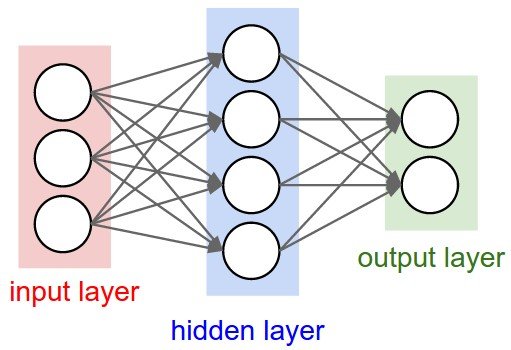
\includegraphics[width=0.6\linewidth]{img/nn/neural_net.jpeg}
  \caption{An sample neural network architecture\todotext{internet...}} 
  \label{fig:sample_nn}
\end{figure}

